\PassOptionsToPackage{sols}{handout}
\documentclass[main]{subfiles}
\setcounterrefbeforedot{chapter}{m-ws3-3}
\setcounterrefafterdot{section}{m-ws3-3}
\addtocounter{section}{-1}
\usepackage{solutions}

\begin{document}

\ifSubfilesClassLoaded{%
  \chaptermark{\chapterthree}
}{}

\section{Inverse Trig Functions} \label{ws3-3}

\begin{problemonly}
    \begin{framed}

\textbf{Key Ideas}:

\begin{itemize}[topsep=0pt,partopsep=0pt,parsep=8pt,itemsep=0pt]

\item You should understand how the inverse trigonometric functions
  $\arcsin x$, $\arccos x$, and $\arctan x$ are defined.  (In particular,
  you should understand that they are not literally inverse functions of
  $\sin x$, $\cos x$, and $\tan x$ because these three functions are not
  invertible.)

\item You should be comfortable using the definitions of $\arcsin x$,
  $\arccos x$, and $\arctan x$ to graph these functions and find their
  domains and ranges.

\item You should understand the difference between the notation $\sin^{-1}
  x$ and $(\sin x)^{-1}$.

\item You should be able to solve basic equations of the form $\sin x =
  a$, $\cos x = a$, and $\tan x = a$ on restricted and unrestricted
  intervals, expressing your solutions using inverse trig functions.

\end{itemize}
\end{framed}
\end{problemonly}

\begin{enumerate}
\item 
  \note{I have this here so that, when we try to define $\arcsin x$, they
    understand why we can't define it to be ``the'' number whose sine is
    $x$.}

  \begin{problem}[\stretch{0.25}]
    \textbf{Warm Up.} Think of two different numbers $\theta$ such that
    $\sin \theta = \frac{1}{2}$.
  \end{problem}

  \begin{solution}
    Two possible answers are $\theta = \frac{\pi}6$ and $\theta =
    \frac{5\pi}{6}$.
  \end{solution}

\item 
  \note{This is motivation for defining inverse trig functions.  It's also
    a true story - the lawyer was Robin's brother-in-law!

    One thing to keep in mind for the next class is that students often
    confuse the idea of solving an equation with that of evaluating a(n
    inverse) function. In this case, the distinction is unimportant
    because the value that the inverse function will spit out is the value
    we want. (Also, we're not going to solve this one.) However, there
    will be cases where we ask them to solve an equation on an unusual
    domain or on a domain in which the equation has two or more
    solutions. I wouldn't get bogged down in this idea yet, but keep it in
    the back of your mind and look for opportunities to point out the
    differences between these two processes/ideas.  }

  \begin{problem}[\stretch{0.75}]
    A New York lawyer is working on the case of an elderly woman who
    twisted her ankle while chasing a runaway shopping cart down a ramp
    outside a Manhattan grocery store.  The curb is 6.5 inches high and
    the flat ground from the edge of the curb to the end of the ramp measures
    50 inches.  New York City law specifies that ramps must have a sloping
    angle of no more than 5 degrees. He needs to know whether the
    construction of this ramp was in accordance with the law.  What
    equation must we solve in order to find the sloping angle of the ramp?
  \end{problem}

  \begin{solution}
    Here's a sketch of the situation, with the angle in question called
    $\theta$:
    \begin{center}
      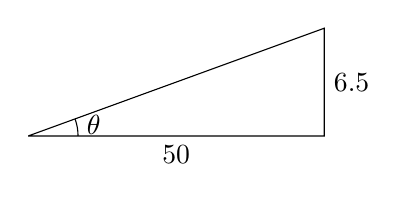
\begin{tikzpicture}
        \draw (0, 0) -- (20:4) -- node[right]{6.5} (20:4 |- 0, 0) --
        node[below]{50} (0, 0);
        \draw (18pt, 0) arc[radius=18pt, start angle=0, end angle=20];
        \draw (10:24pt) node{$\theta$};
      \end{tikzpicture}
    \end{center}
    From the sketch, we can see that $\tan \theta = \frac{6.5}{50}$; we'd
    like to solve this equation for $\theta$. 
  \end{solution}

\item Recall what you know about invertibility and inverse functions
  from Math Ma.
  \begin{itemize}[topsep=0pt]
    \item
    \begin{problem}[\stretch{0.25}]
    What is key in order for a function to be invertible?
    \end{problem}

    \begin{solution}
      The function has to be one-to-one.
      The graph has to pass
      the horizontal line test.
    \end{solution}

    \item
    \begin{problem}[\stretch{0.25}]
    If a function is invertible, how can we find $f^{-1}(x)$?
    \end{problem}

    \begin{solution}
        Switch $x$ and $y$ in $y=f(x)$ and
        solve for $y$.
    \end{solution}

    \item
    \begin{problem}[\stretch{0.25}]
    If $(a,b)$ is a point on the graph of $f$, what's the `corresponding'
    point on the graph of $f^{-1}$?
    \end{problem}

    \begin{solution}
        $f^{-1}$ reverses the input-output
        relationship, so $(b,a)$.
    \end{solution}

    \item
    \begin{problem}[\stretch{0.25}]
    What's the relationship between the graph of $f$ and the graph of 
    $f^{-1}$?
    \end{problem}

    \begin{solution}
        They are reflections of each other
        over the line $y=x$.
    \end{solution}
  \end{itemize}
  
  \begin{problem}[\stretch{0.25}]
  What's the biggest obstacle in ``undoing" sine, cosine, and tangent?
  \end{problem}

  \begin{solution}
      They are not invertible since the
      graphs don't pass the horizontal line
      test.
  \end{solution}

\newpage

\item  \note{We'll do this as a class. In fact, you may find that you need
    to do or go over a lot of this worksheet as a class, or keep checking in
    as a class, both because they find it challenging and because you want to clarify.}

  \textit{Defining arcsin.}

  \begin{enumerate}
  \item
    \begin{problem}
      On the axes below, sketch $y = \sin x$, and state the domain and
      range of the function $\sin x$. 
    \end{problem}

    \begin{problemonly}
    \begin{center}
    \begin{tikzpicture}
    \begin{axis}[xlabel=$x$, ylabel=$y$, 
            xmin=-4.8,xmax=4.8,ymin=-3.5,ymax=3.5,
            xtick={-3*pi/2,-pi, -pi/2, pi/2, pi, 3*pi/2},
            xticklabels={$-\frac{3\pi}{2}$, $-\pi$, $-\frac{\pi}{2}$, 
            $\frac{\pi }{2}$, $\pi$, $\frac{3\pi}{2}$},
            ytick={-3.14159, -1.5708, 0., 1.5708, 3.14159},
            yticklabels={$-\pi$, $-\frac{\pi
            }{2}$, $0.$, $\frac{\pi }{2}$, $\pi$},
            minor xtick = {-4,-3,-2,-1,1,2,3,4},
            minor ytick = {-3,-2,-1,1,2,3},
            minor tick length=5pt, minor tick style = {red},
            unit vector ratio*=1 1, width=5.5in]
            \addplot[draw=none] coordinates {(0,0)};
            \pgfplotsinvokeforeach{-4,-3,-2,-1,1,2,3,4}{
            \path (#1,0) node[text=red,above] {\footnotesize#1};
            \path (0,#1) node[text=red,right] {\footnotesize#1};
            }
    \end{axis}
    \end{tikzpicture}
    \end{center}

    \begin{center}
    \begin{tabular}{ccc}
    Domain of $\sin x$: $\fitb{1in}{(-\infty, \infty)}$
    &&
    Range of $\sin x$: $\fitb{1in}{[-1, 1]}$
    \end{tabular}
    \end{center}
    \end{problemonly}

    

    \begin{solution}
      Here's the graph of $\sin x$; its domain is $(-\infty, \infty)$, and
      its range is $[-1, 1]$.
      \begin{center}
        \begin{tikzpicture}
          \begin{axis}[xlabel=$x$, ylabel=$y$,
            xmin=-4.8,xmax=4.8,ymin=-3.5,ymax=3.5,
            xtick={-3*pi/2,-pi, -pi/2, pi/2, pi, 3*pi/2},
            xticklabels={$-\frac{3\pi}{2}$, $-\pi$, $-\frac{\pi}{2}$, 
            $\frac{\pi }{2}$, $\pi$, $\frac{3\pi}{2}$},
            ytick={-3.14159, -1.5708, 0., 1.5708, 3.14159},
            yticklabels={$-\pi$, $-\frac{\pi
            }{2}$, $0.$, $\frac{\pi }{2}$, $\pi$},
            minor xtick = {-4,-3,-2,-1,1,2,3,4},
            minor ytick = {-3,-2,-1,1,2,3},
            minor tick length=5pt, minor tick style = {red},
            unit vector ratio*=1 1, width=5.5in]
            \addplot[draw=none] coordinates {(0,0)};
            \pgfplotsinvokeforeach{-4,-3,-2,-1,1,2,3,4}{
            \path (#1,0) node[text=red,above] {\footnotesize#1};
            \path (0,#1) node[text=red,right] {\footnotesize#1};
            }
            \addplot[black] {sin(deg(x))};
          \end{axis}
        \end{tikzpicture}
      \end{center}
    \end{solution}

    \item
    \begin{problem}[\vfill]
      We would \textit{like} to define $\arcsin x$ to be the inverse
      function of $\sin x$.  Why can't we do that?
    \end{problem}

    \begin{solution}
      \answer{$\sin x$ is not an invertible function (it fails the
        horizontal line test).}
    \end{solution}

  \item
    \begin{problem}[\vfill]
      Can we restrict $\sin x$ to an interval on which it is invertible?  
    \end{problem}

    \begin{solution}
      \answer{If we restrict $\sin x$ to the interval $\left[
          -\frac{\pi}{2}, \frac{\pi}{2}\right]$, then it is invertible
        on this restricted domain.  (This is not the only possible
        interval; for example, if we restrict $\sin x$ to $\left[
          \frac{\pi}{2}, \frac{3 \pi}{2} \right]$, this restriction
        would also be invertible.  However, $\left[ -\frac{\pi}{2},
          \frac{\pi}{2}\right]$ is the interval that mathematicians have
        agreed on for defining $\arcsin$.)}
    \end{solution}

  \item

    \note{This can be challenging.  Even though students probably
      remember that they can sketch inverse functions by reflecting over
      $y = x$, many find this hard to do.  Help them with strategies,
      such as plotting a few points they know.}

    \begin{problem}
      If we restrict $\sin x$ to the interval $ \left[ -
        \frac{\pi}{2}, \frac{\pi}{2} \right]$, then it is invertible;
      we'll define $\arcsin x$ to be the inverse of this restricted
      function. $\arcsin x$ is the angle in the interval $[-\frac{\pi}{2},
      \frac{\pi}{2}]$ whose sine is $x$.
      
      On the axes above, sketch $y = \arcsin x$.  To guide
      yourself, label 3 points on the graph of
      $\sin x$ in the interval $[-\frac{\pi}{2},\frac{\pi}{2}]$. To graph
      $\arcsin x$, you can plot the corresponding points.
      
      What are the domain and range of the function $\arcsin x$?
      \begin{center}
      \begin{tabular}{ccc}
        Domain of $\arcsin x$: $\fitb{1in}{[-1,1]}$
        &&
        Range of $\arcsin x$: $\fitb{1in}{[-\frac{\pi}{2},\frac{\pi}{2}]}$
      \end{tabular}
      \end{center}
    \end{problem}

    \begin{solution}
      First, here's the restriction of $\sin x$ to $\displaystyle \left[ -
        \frac{\pi}{2}, \frac{\pi}{2} \right]$:
      \begin{center}
        \begin{tikzpicture}
          \begin{axis}[xlabel=$x$, ylabel=$y$,
            xmin=-3.5,xmax=3.5,ymin=-3.5,ymax=3.5,
            xtick={-3.14159, -1.5708, 0., 1.5708, 3.14159},
            xticklabels={$-\pi$, $-\frac{\pi}{2}$, $0.$, $\frac{\pi }{2}$, $\pi$},
            ytick={-3.14159, -1.5708, 0., 1.5708, 3.14159},
            yticklabels={$-\pi$, $-\frac{\pi
            }{2}$, $0.$, $\frac{\pi }{2}$, $\pi$},
            minor tick = {-3,-2,-1,1,2,3},
            minor tick length=5pt, minor tick style = {red},
            unit vector ratio=1 1, width=4in]
            \addplot[draw=none] coordinates {(0,0)};
            \pgfplotsinvokeforeach{-3,-2,-1,1,2,3}{
            \path (#1,0) node[text=red,above] {\footnotesize#1};
            \path (0,#1) node[text=red,right] {\footnotesize#1};
            }
            \addplot+[domain=-pi/2:pi/2, black]{sin(deg(x))} node[right]
            {$\sin x$};
            \addplot[closed] coordinates {(-pi/2,-1) (0,0) (pi/2,1)};
          \end{axis}
        \end{tikzpicture}
      \end{center}
      The inverse of this is the red graph:      
      \begin{center}
        \answer{
          \begin{tikzpicture}
            \begin{axis}[xlabel=$x$, ylabel=$y$,
            xmin=-3.5,xmax=3.5,ymin=-3.5,ymax=3.5,
            xtick={-3.14159, -1.5708, 0., 1.5708, 3.14159},
            xticklabels={$-\pi$, $-\frac{\pi}{2}$, $0.$, $\frac{\pi }{2}$, $\pi$},
            ytick={-3.14159, -1.5708, 0., 1.5708, 3.14159},
            yticklabels={$-\pi$, $-\frac{\pi
            }{2}$, $0.$, $\frac{\pi }{2}$, $\pi$},
            minor tick = {-3,-2,-1,1,2,3},
            minor tick length=5pt, minor tick style = {red},
            unit vector ratio=1 1, width=4in]
            \addplot[draw=none] coordinates {(0,0)};
            \pgfplotsinvokeforeach{-3,-2,-1,1,2,3}{
            \path (#1,0) node[text=red,above] {\footnotesize#1};
            \path (0,#1) node[text=red,right] {\footnotesize#1};
            }
              \addplot+[domain=-pi/2:pi/2, black]{sin(deg(x))} node[right]
              {$\sin x$};
              \addplot+[domain=-1:1, red]{rad(asin(x))}
              node[above]{$\arcsin x$};
              \addplot[closed] coordinates {(-pi/2,-1) (0,0) (pi/2,1)};
              \addplot[closed, red] coordinates {(-1,-pi/2) (0,0) (1,pi/2)};
            \end{axis}
          \end{tikzpicture}
        }
      \end{center}
      From this, we can see that \fbox{the domain of $\arcsin x$ is
        $[-1, 1]$, and the range is $\left[ - \frac{\pi}{2},
          \frac{\pi}{2} \right]$.}
    \end{solution}

    \pspace{\newpage}

  \item

    \begin{problem}[0.1in]
      \answer{If $P = \arcsin Q$, how could you express $Q$ in terms of $P$?
        $\fitb{1in}{Q = \sin P}$}
    \end{problem}

    \begin{solution} 
      Graphically, saying that $P = \arcsin Q$ is saying that $(Q, P)$
      is a point on the graph of $y = \arcsin x$.  Therefore, $(P, Q)$
      is a point on the portion of $y = \sin x$ with $- \frac{\pi}{2}
      \leq x \leq \frac{\pi}{2}$.  In other words, $Q = \sin P$ and $P$
      is in the interval $\left[ - \frac{\pi}{2}, \frac{\pi}{2}
      \right]$. 
    \end{solution}

    \begin{problem}[\vfill]
      \answer{In words, $\arcsin Q$ is \fitb{4.5in}{the angle in
          $\displaystyle \left[ - \dfrac{\pi}{2}, \dfrac{\pi}{2} \right]$
          whose sine is $Q$}.}
    \end{problem}

    \note{It's worth looking again at the domain and range in terms of
      the verbal description of $\arcsin x$.}

  \item
    \begin{problem}[\vfill]
      What is $\arcsin \left( \frac{1}{2} \right)$?  
    \end{problem}

    \begin{solution}
      By definition, it's the angle in $\left[ - \frac{\pi}{2},
        \frac{\pi}{2} \right]$ whose sine is $\frac{1}{2}$.  In other
      words, we are trying to think of the (only!) angle $\theta$ in
      $\left[ - \frac{\pi}{2}, \frac{\pi}{2} \right]$ such that $\sin
      \theta = \frac{1}{2}$.  This angle is $\theta =
      \boxed{\frac{\pi}{6}}$.
    \end{solution}

  \end{enumerate}

  \begin{problemonly}
    \begin{framed}
      \settowidth{\dwidth}{\Large{\fontencoding{U}\fontfamily{futs}\selectfont\char 49\relax}} {\Large{\fontencoding{U}\fontfamily{futs}\selectfont\char 49\relax}}
      \begin{minipage}[t]{\linewidth-\dwidth-2\fboxsep}
        The function $\arcsin x$ is also written as $\sin^{-1} x$.  It's
        important to remember that $\sin^{-1} x$ refers to $\arcsin x$,
        \textit{not} to $(\sin x)^{-1}$; $(\sin x)^{-1}$ is the same as
        $\frac{1}{\sin x}$, which is the same as $\csc x$.  (Yes, this
        notation is inconsistent: $\sin^2 x$ \emph{is} the same thing as
        $(\sin x)^2$.  This is one of those quirks that you just have to
        remember!)
      \end{minipage}
    \end{framed}
  \end{problemonly}

  \begin{enumerate}[resume]

  \item

    \begin{problem}[\vfill]
      True or false: since $\sin \left( \frac{11 \pi}{6} \right) = -
      \frac{1}{2}$, $\sin^{-1} \left( - \frac{1}{2} \right) = \frac{11
        \pi}{6}$. 
    \end{problem}

    \begin{solution}
      \fbox{False.}  Although it's true that $\sin \left( \frac{11 \pi}{6}
      \right) = - \frac{1}{2}$, $\sin^{-1} \left( -\frac{1}{2} \right)$ is
      defined to be the angle \hl{\textbf{in $\bm{\left[- \frac{\pi}{2},
              \frac{\pi}{2} \right]}$}} whose sine is $- \frac{1}{2}$, and
      $\frac{11 \pi}{6}$ is not in the interval $\left[- \frac{\pi}{2},
        \frac{\pi}{2} \right]$.  The (only!) angle in $\left[-
        \frac{\pi}{2}, \frac{\pi}{2} \right]$ whose sine is $-
      \frac{1}{2}$ is $- \frac{\pi}{6}$, so the correct statement is
      $\boxed{\sin^{-1} \left( - \frac{1}{2} \right) = -\frac{\pi}{6}}$.
    \end{solution}

  \end{enumerate}

\item 
  \note{Mostly, the goal here is to agree on the ranges or $\arccos x$ and
    $\arctan x$, as well as to give them some practice graphing an inverse
    trig function.}

  Similarly, we'll define:
  \begin{itemize}
  \item $\arccos x = {}$ \solonly{\textbf{the angle in the interval
        $\bm{[0, \pi]}$ whose cosine is $\bm{x}$}}

  \item $\arctan x = {}$ \solonly{\textbf{the angle in the interval
        $\bm{\left(-\frac{\pi}{2}, \frac{\pi}{2} \right)}$ whose tangent
        is $\bm{x}$}}
  \end{itemize}

  Graph $\arctan x$.  What are its domain and range?

  \begin{problemonly}
    \begin{tabular}{c c c}
      \parbox[t]{2.85in}{\vspace{0pt}
        \axes[xtick={-4.71239, -3.14159, -1.5708, 0., 1.5708, 3.14159,
          4.71239}, xticklabels={$-\frac{3 \pi }{2}$, $-\pi$, $-\frac{\pi
          }{2}$, $0.$, $\frac{\pi }{2}$, $\pi$, $\frac{3 \pi }{2}$},
        ytick={-4.71239, -3.14159, -1.5708, 0., 1.5708, 3.14159, 4.71239},
        yticklabels={$-\frac{3 \pi }{2}$, $-\pi$, $-\frac{\pi
          }{2}$, $0.$, $\frac{\pi }{2}$, $\pi$, $\frac{3 \pi }{2}$},
        xmin=-4.8, xmax=5, ymin=-4.8, ymax=5]
      }
      & &
      \parbox[t]{2.5in}{%
        \setlength{\parskip}{16pt}

        \vspace*{32pt}

        Domain of $\arctan x$: $\fitb{1in}{(-\infty, \infty)}$

        Range of $\arctan x$: $\fitb{1in}{\left(-\frac{\pi}{2},
            \frac{\pi}{2} \right)}$
      }
    \end{tabular}
  \end{problemonly}

  \begin{solution}
    Here's the restriction of $\tan x$ to $\left( -\frac{\pi}{2},
      \frac{\pi}{2} \right)$:   
    \begin{center}
      \begin{tikzpicture}
        \begin{axis}[xtick=\empty, extra x ticks={-1.5708, 1.5708}, extra
          x tick labels={$-\frac{\pi}{2}$, $\frac{\pi}{2}$}, ytick=\empty,
          xmin=-4.25, xmax=4.25, ymin=-4.25, ymax=4.25, width=3in,
          height=3in] %
          \addplot+[domain=-pi/2:pi/2, red, restrict y to
          domain=-5:5]{tan(deg(x))} node[above] {$\tan x$};
        \end{axis}
      \end{tikzpicture}
    \end{center}
    $\arctan x$ is the inverse of the graph above.
    \begin{center}
      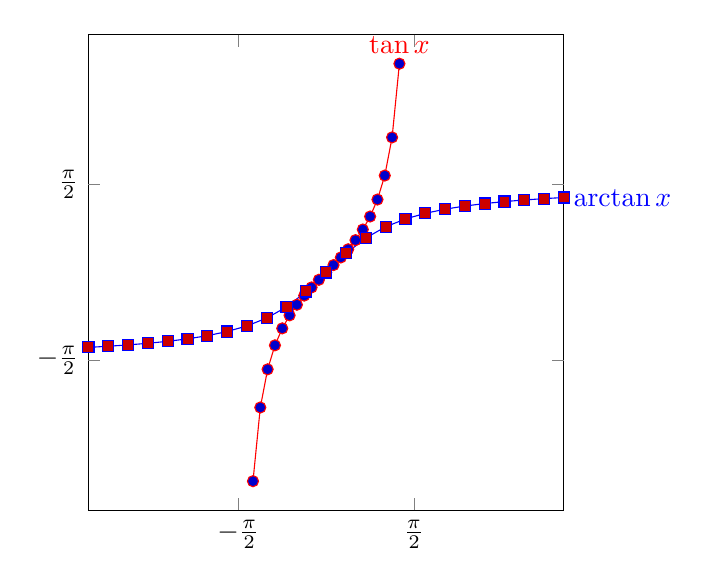
\begin{tikzpicture}
        \begin{axis}[xtick=\empty, extra x ticks={-1.5708, 1.5708}, extra
          x tick labels={$-\frac{\pi}{2}$, $\frac{\pi}{2}$}, ytick=\empty,
          extra y ticks={-1.5708, 1.5708}, extra y tick
          labels={$-\frac{\pi}{2}$, $\frac{\pi}{2}$}, xmin=-4.25,
          xmax=4.25, ymin=-4.25, ymax=4.25, width=3in, height=3in,
          clip=false] %  
          \addplot+[domain=-pi/2:pi/2, red, restrict y to
          domain=-5:5]{tan(deg(x))} node[above] {$\tan x$}; %
          \addplot+[blue, solid, domain=-4.25:4.25]{rad(atan(x))} node[right]{$\arctan x$};
        \end{axis}
      \end{tikzpicture}
    \end{center}
    As we can see from the graph, \fbox{the domain of $\arctan x$ is
      $(-\infty, \infty)$, and the range is $\left( - \frac{\pi}{2},
        \frac{\pi}{2} \right)$}.
  \end{solution}

  \begin{framed}
    Although we call $\arcsin x$, $\arccos x$, and $\arctan x$
    \textit{inverse trigonometric functions}, remember that they are not
    really the inverse functions of $\sin x$, $\cos x$, and $\tan x$
    (because $\sin x$, $\cos x$, and $\tan x$ are not invertible!).  They
    are only the inverse functions of $\sin x$, $\cos x$, and $\tan x$
    \emph{when each function's domain is restricted in a certain way}.
  \end{framed}
\end{enumerate}

\begin{enumerate}[resume]

\item 
\begin{problem}[\vfill\newpage]
Return to problem 2 about the New York ramp. Was the ramp within legal guidelines?
\end{problem}

\begin{solution} The angle of the ramp is $\arctan(6.5/50)\approx\ang{7.4}$.
The ramp is not within legal guidelines.
\end{solution}

\item
\begin{enumerate}
  \item
  \begin{problem}Evaluate each of the following:
  
  \begin{multicols}{2}
    \begin{enumerate}[topsep=0pt]
      \item $\sin(\arcsin(0.5))\solonly{=0.5}$
      \columnbreak
      \item $\arcsin(\sin(0.5))\solonly{=0.5}$
    \end{enumerate}
  \end{multicols}
  \vspace{-6pt}
  \end{problem}

  
  \item 
  \begin{problem}[\stretch{0.5}]
  Which of the following is undefined, and why?
  
  \begin{multicols}{2}
    \begin{enumerate}[topsep=0pt]
      \item $\arcsin(-0.2)$
      \columnbreak
      \item $\arcsin(2)$
    \end{enumerate}
  \end{multicols}
  \end{problem}
  
  \begin{solution}
    $\arcsin{2}$ is undefined because the domain
    of $\arcsin x$ is $[-1,1]$, and there is no real number whose sine is 2.
  \end{solution}


\item 
  \note{This is to emphasize that $\sin$ and $\arcsin$ are not really
    inverse functions in the way they may expect.  (When we compose them,
    we don't get just the identity.)}

  \begin{problem}[\stretch{0.5}]
  Which of the two expressions below is not defined? Why not? The other
  \textbf{is} defined. Evaluate it.
  
    \begin{multicols}{2}
    \begin{enumerate}
    \item
        $\displaystyle \arcsin \left(\sin \frac{3 \pi}{2} \right)$
      
    \columnbreak
    
    \item
        $\displaystyle \sin \left( \arcsin \frac{3 \pi}{2} \right)$

    \end{enumerate}
    \end{multicols}
    \end{problem}

    \begin{solution}
    $\displaystyle \sin \left( \arcsin \frac{3 \pi}{2} \right)$ is
        undefined because $ \arcsin \frac{3 \pi}{2}$ is undefined. There
        is no angle whose sine is  $ \frac{3 \pi}{2}$.  (This is
        consistent with the fact that the domain of $\arcsin x$ is $[-1,
        1]$, since $\frac{3 \pi}{2}$ it outside that interval.)
        Since $\sin \frac{3 \pi}{2} = -1$, this is asking for
        $\arcsin(-1)$.  That's defined to be the angle in $\left[ -
          \frac{\pi}{2}, \frac{\pi}{2} \right]$ with sine value $-1$, and
        the single such angle is $\boxed{ -\frac{\pi}{2}}$.
    \end{solution}
    \end{enumerate}

\item 
  \emph{Using inverse trig functions to solve equations.}

  \begin{enumerate}
  \item

    \note{They have done problems like this already, but I want to do one
      ``concrete'' example before getting into ones that require inverse
      trig functions.}

    \begin{problem}[\stretch{1}]
      Find all values of $x$ in $[0, 2 \pi]$ such that $\tan x = 1$; give exact answers.
    \end{problem}

    \begin{solution}
      There are two:
      \begin{center}
        \begin{tikzpicture}
        \begin{axis}[axis equal=true, 
          xmin=-1.2, xmax=1.2, ymin=-1.2, ymax=1.2, clip=false,
          xtick=\empty, ytick=\empty, width=3in]
          \coordinate (O) at (0,0);
          \coordinate (A) at (1,0);
          \coordinate (R) at (\rtheta{1}{45});
          \coordinate (P) at (\rtheta{1}{225});
          \addplot[domain=0:360, data cs=polar] (x,1);
          \draw[thick,blue] (O) -- (R);
          \draw[thick,red] (O) -- (P);
          \filldraw[fill=blue,radius=2pt] (R) circle;
          \filldraw[fill=red,radius=2pt] (P) circle;
          \draw pic[text=blue,draw=blue,thick,angle radius=15,
          "\normalsize$\frac{\pi}{4}$",angle eccentricity=1.5]
          {angle=A--O--R};
          \draw pic[text=red,draw=red,thick,angle radius=10,
          "\normalsize$\frac{5\pi}{4}$",angle eccentricity=1.9]
          {angle=A--O--P};
        \end{axis}
      \end{tikzpicture}
      \end{center}
    \end{solution}

  \item

    \note{This is \emph{very} hard, and you'll probably want to do this
      together just so that students understand that finding the angles
      ``exactly'' means writing them in terms of
      $\arctan\left(\frac{1}{3}\right)$.}

    \begin{problem}[\stretch{1}]
      Find all values of $x$ in $[0, 2 \pi]$ such that $\tan x =
      \frac{1}{3}$; give exact answers (which will involve inverse
      trigonometric functions).
    \end{problem}

    \begin{solution}
      One solution of the equation $\tan x = \frac{1}{3}$ is $x = \arctan
      \frac{1}{3}$.  For short, let's call this $A$.  Remember that $A =
      \arctan \frac{1}{3}$ is the angle in $\left( - \frac{\pi}{2},
        \frac{\pi}{2} \right)$ whose tangent is $\frac{1}{3}$; it is the blue
        angle below. (In particular, since $A$ must be in $\left( - \frac{\pi}{2},
        \frac{\pi}{2} \right)$ and $\tan A$ is positive, $A$ is between
      $0$ and $\frac{\pi}{2}$.)
      
      Now, we can picture all values of $x$ in
      $[0, 2 \pi]$ such that $\tan x = \frac{1}{3}$ and express these in
      terms of $A$.  The other possible angle is shown in red.
      So, there are two values of $x$,
      $\boxed{\arctan\left(\tfrac{1}{3}\right) \text{ and } \pi +
        \arctan\left(\tfrac{1}{3}\right)}$. 
      \begin{center}
        \begin{tikzpicture}
        \begin{axis}[axis equal=true, 
          xmin=-1.3, xmax=1.3, ymin=-1.3, ymax=1.3, clip=false,
          xtick=\empty, ytick=\empty, width=3in]
          \coordinate (O) at (0,0);
          \coordinate (A) at (1,0);
          \coordinate (R) at (\rtheta{1}{18.43});
          \coordinate (P) at (\rtheta{1}{198.43});
          \addplot[domain=0:360, data cs=polar] (x,1);
          \addplot[domain=-1.3:1.3,dashed,black] {x/3}
          node[below] {$y=\frac{1}{3}x$};
          \draw[thick,blue] (O) -- (R);
          \draw[thick,red] (O) -- (P);
          \filldraw[fill=blue,radius=2pt] (R) circle;
          \filldraw[fill=red,radius=2pt] (P) circle;
          \draw pic[text=blue,draw=blue,thick,angle radius=18,
          "\normalsize$A$",angle eccentricity=1.6]
          {angle=A--O--R};
          \draw pic[text=red,draw=red,thick,angle radius=10,
          "\normalsize$\pi+A$",angle eccentricity=1.6]
          {angle=A--O--P};
        \end{axis}
      \end{tikzpicture}
      \end{center}
    \end{solution}

  \item
    \begin{problem}[\stretch{1}]
      Solve $\cos x = -0.7$ on $[0, 2 \pi]$. Use the unit circle or
      graph of $\cos x$ to ensure you have all solutions.
    \end{problem}

    \begin{solution}
      One solution of $\cos x = -0.7$ is $x = \arccos (-0.7)$.  For short,
      let's call this $A$.  Remember that $A = \arccos(-0.7)$ is the angle
      in $[0, \pi]$ whose cosine is $-0.7$; it is the blue angle below.
      (In particular, since $A$ must be in $[0, \pi]$ and $\cos A$ is
      negative, $A$ is between $\frac{\pi}{2}$ and $\pi$.) 
      
      Now, we can
      picture all values of $x$ in $[0, 2 \pi]$ such that $\cos x = -0.7$
      and express these in terms of $A$.  The other possible angle is
      shown below in red. So, there are two values of $x$, $\boxed{\arccos(-0.7) \text{ and }
        2 \pi - \arccos(-0.7)}$. 
      \begin{center}
      \begin{tikzpicture}
        \begin{axis}[axis equal=true, 
          xmin=-1.3, xmax=1.3, ymin=-1.3, ymax=1.3, clip=false,
          xtick=\empty, ytick=\empty, extra x ticks={-0.7}, width=3in,
          set layers=tick labels on top]
          \coordinate (O) at (0,0);
          \coordinate (A) at (1,0);
          \coordinate (R) at (\rtheta{1}{134.4});
          \coordinate (P) at (\rtheta{1}{225.6});
          \addplot[domain=0:360, data cs=polar] (x,1);
          \draw[thick,blue] (O) -- (R);
          \draw[thick,red] (O) -- (P);
          \filldraw[fill=blue,radius=2pt] (R) circle;
          \filldraw[fill=red,radius=2pt] (P) circle;
          \draw pic[text=blue,draw=blue,thick,angle radius=18,
          "\normalsize$A$",angle eccentricity=1.4]
          {angle=A--O--R};
          \draw pic[text=red,draw=red,thick,angle radius=10]
          {angle=A--O--P};
          \draw[->,draw=red,text=red] (-1,0.5) node[left] {$2\pi-A$}
          to (-0.2,0.1);
        \end{axis}
      \end{tikzpicture}
      \end{center}
      
    \end{solution}

  \item
    \note{The big point here is that $\arcsin \left( - \frac{1}{4}
      \right)$ is \emph{not} one of the angles we want. Even after
      acknowledging this, students will have trouble remembering and
      dealing with the fact that $\arcsin \left( - \frac{1}{4}\right)$ is
      negative.  Some students may find it easier to write the solutions
      in terms of $\arcsin \left( \frac{1}{4} \right)$, so it can be nice
      to discuss it both ways.}

    \begin{problem}[\stretch{1}]
      Solve $\sin x = - \frac{1}{4}$ on $[0, 2 \pi]$. Use the unit circle
      or graph of $\sin x$ to ensure you have all solutions.
    \end{problem}

    \begin{solution}
      We know one solution to $\sin x = -\frac{1}{4}$, $x = \arcsin \left(
        -\frac{1}{4} \right)$.  For short, let's call this $A$.  Remember
      that $A = \arcsin \left( -\frac{1}{4} \right)$ is the angle in
      $\left[ - \frac{\pi}{2}, \frac{\pi}{2} \right]$ whose sine is
      $-\frac{1}{4}$; we can picture it like this:
      \begin{center}
        \begin{tikzangle}[angle=rad(asin(-1/4)), label=$\ A$, color=blue,
          func=sin, functick=$-\frac{1}{4}$] %
          \draw[blue] (axis cs: 1.5, 0) node[right] {$A = \arcsin \left(
              -\frac{1}{4} \right)$};
        \end{tikzangle}
      \end{center}
      (In particular, since $A$ must be in $\left[ - \frac{\pi}{2},
        \frac{\pi}{2} \right]$ and $\sin A$ is negative, $A$ is between
      $-\frac{\pi}{2}$ and $0$.)

      Because $A$ is negative, many people find it easier to work in terms
      of $B = \arcsin \left( \frac{1}{4} \right)$, which is between $0$
      and $\frac{\pi}{2}$; we can picture $B$ like this:
      \begin{center}
        \begin{tikzangle}[angle=rad(asin(1/4)), label=$\ B$, color=blue,
          func=sin, functick=$\frac{1}{4}$] %
          \draw[blue] (axis cs: 1.5, 0) node[right] {$B = \arcsin \left(
              \frac{1}{4} \right)$};
        \end{tikzangle}
      \end{center}
      (From our diagrams, we can see that $B = -A$.)

      There are two angles in $[0, 2 \pi]$ such that $\sin x = -
      \frac{1}{4}$; we can express them in terms of $A$ or $B$:
      \begin{center}
        \begin{tabular}{ccc}
          \begin{tikzangle}[angle=pi+rad(asin(1/4)), func=sin,
            functick=$-\frac{1}{4}$, label=$x$,
            labelpos=0.6] % 
          \end{tikzangle}
          &&
          \begin{tikzangle}[angle=2*pi-rad(asin(1/4)), func=sin,
            functick=$-\frac{1}{4}$, label=$x$,
            labelpos=0.4] % 
          \end{tikzangle}
          \\
          $\displaystyle
          \begin{aligned}
            x &= \pi + B \\
            &= \pi - A            
          \end{aligned}$
          && $\displaystyle
          \begin{aligned}
            x &= 2 \pi - B \\
            &= 2 \pi + A            
          \end{aligned}$
        \end{tabular} 
      \end{center}
      So, the two values of $x$ are $\boxed{ \pi + \arcsin \left(
          \tfrac{1}{4} \right) \text{ and } 2 \pi - \arcsin \left(
          \tfrac{1}{4} \right)}$.  Alternatively, these could be expressed
      as $\pi - \arcsin \left( - \frac{1}{4} \right)$ and $2 \pi + \arcsin
      \left( - \frac{1}{4} \right)$.  (If you plug these in a calculator,
      they are $\approx 3.39$ and $\approx 6.03$.)

      \emph{Note:} It may seem surprising that $\arcsin \left( -
        \frac{1}{4} \right)$ is not one of the values we want, but
      remember that we figured out that it's negative (and therefore not
      in $[0, 2 \pi]$).
    \end{solution}

  \end{enumerate}

  \pspace{\newpage}

  \item 

  \begin{problem}[\stretch{0.5}]
    Patrick is attempting to simplify $\arctan \left(\tan \frac{3\pi}{4}
    \right)$. He says:
    \begin{quote}
      I know that $\frac{3\pi}{4}$ is in the second quadrant, and its
      reference angle is $45^\circ$, so $\tan \frac{3\pi}{4} = -1$.  So,
      the question is asking me for $\arctan (-1)$.  I know that
      $\arctan$ always gives an angle in the first quadrant or the
      fourth quadrant, and since $-1$ is negative, I'm looking for an
      angle in the fourth quadrant.  I know that $\frac{7 \pi}{4}$ is an
      angle in the fourth quadrant whose tangent is $-1$, so
      $\arctan(\tan \frac{3\pi}{4})=\frac{7\pi}{4}$.
    \end{quote}
    Patrick is not correct. Where does his reasoning go wrong?
  \end{problem}  

  \begin{solution}
    Although it's true that $\arctan$ gives an
    angle in the first or fourth quadrant, that's not specific enough;
    for example, $\frac{\pi}{4}$ and $\frac{9 \pi}{4}$ have the same
    terminal side in the first quadrant, but they are not the same
    number.  The more precise statement is that $\arctan$ gives an angle
    in the interval $\left( - \frac{\pi}{2}, \frac{\pi}{2} \right)$, so
    $\arctan(-1) = - \frac{\pi}{4}$, not $\frac{7 \pi}{4}$.
  \end{solution}

  \item
    \begin{problem}[\vfill]
      Find all values of $x$ such that $\tan x = 2$.
    \end{problem}

    \begin{solution}
      One solution of $\tan x = 2$ is $\arctan 2$; let's call this $A$ for
      short.  By definition, it's the angle in $\left( - \frac{\pi}{2},
        \frac{\pi}{2} \right)$ whose tangent is 2.  We can visualize $A =
      \arctan 2$ like this:
      \begin{center}
        \begin{tikzangle}[angle=rad(atan(2)), label=$A$]
          \draw[red] (axis cs: \px, \py) node[anchor=south west, text width=1in]{terminal side has
            slope 2};
        \end{tikzangle}
      \end{center}
      When we're solving $\tan x = 2$, we're trying to think of all angles
      whose terminal side has slope 2; that's all angles that end on
      either the green or blue segment below:
      \begin{center}
        \begin{tikzangle}[angle=rad(atan(2)), label=$A$]
          \draw[green!70!black] (axis cs: 0, 0) -- (axis cs: \px, \py);
          \draw[blue] (axis cs: 0, 0) -- (axis cs: -\px, -\py);
        \end{tikzangle}
      \end{center}
      We can see that such angles are simply $A$ plus an integer multiple
      of $\pi$, so the solutions of $\tan x = 2$ are \fbox{$\pi n +
        \arctan 2$ where $n$ is any integer} (that is, $\arctan 2$ plus
      any integer multiple of $\pi$).

      Alternatively, you could think about this in terms of the graph of
      $\tan x$; unlike $\sin$ and $\cos$, $\tan x$ has period $\pi$.  We
      can see from the graph that the solutions of $\tan x = 2$ (marked on
      the $x$-axis in red) are spaced exactly $\pi$ apart:
      \begin{center}
        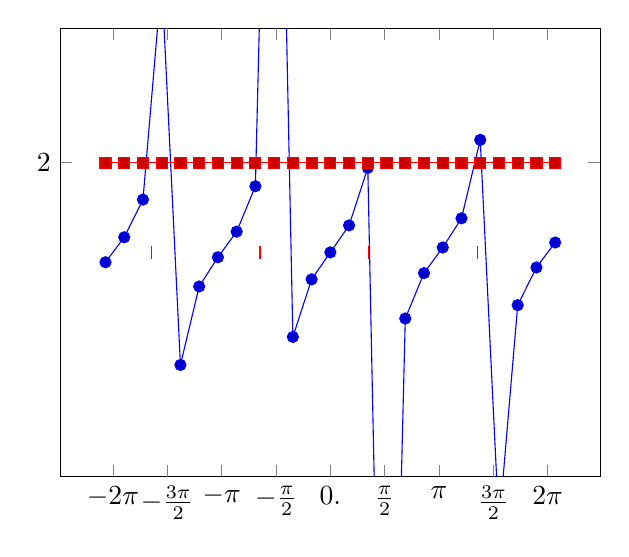
\begin{tikzpicture}
          \begin{axis}[xtick={-6.28319, -3.14159, 0., 3.14159, 6.28319},
            xticklabels={$-2 \pi$, $-\pi$, $0.$, $\pi$, $2 \pi$}, ymin=-5,
            ymax=5, ytick={2}, extra x ticks={-4.71239, -1.5708, 1.5708,
              4.71239}, extra x tick labels={$-\frac{3 \pi }{2}$,
              $-\frac{\pi }{2}$, $\frac{\pi }{2}$, $\frac{3 \pi }{2}$}]
            \addplot+[domain=-6.5:6.5, restrict y to domain=-20:20]{tan(deg(x))};
            \addplot+[domain=-6.5:6.5]{2};
            \pgfplotsforeachungrouped \x in {1.10715, -5.17604, -2.03444,
              4.24874}
            {
              \edef\temp{\noexpand\draw[red] (axis cs: \x, 0.15) -- (axis cs:
                \x, -0.15);}
              \temp
            }
          \end{axis}          
        \end{tikzpicture}
      \end{center}
    \end{solution}

  \end{enumerate}

\solonly{\newpage}

\begin{framed}
\textbf{What we've learned:}
\begin{itemize}[topsep=0pt]
  \item The only way we can ``undo" the periodic trig functions is to
    restrict their domains so they're 1-to-1.
  \item The restrictions are \emph{conventions}. Convince yourself
    they are natural conventions.
    \begin{center}
    \begin{tabular}{ccc}
        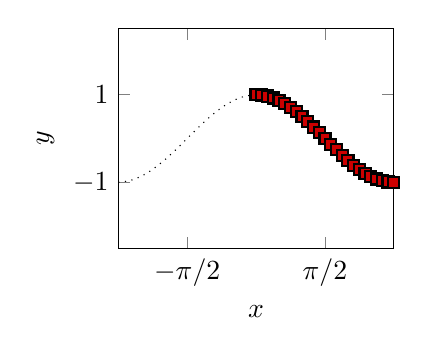
\begin{tikzpicture}
          \begin{axis}[width = 2in,
            xmin=-pi, xmax=pi, ymin=-1.2,ymax=1.2,
            xtick={-pi/2,pi/2}, xticklabels={$-\pi/2$,$\pi/2$},
            ytick={-1,1}, xlabel=$x$, ylabel=$y$, axis equal=true]
            \addplot[domain=-pi:pi,dotted,black]{cos(deg(x))};
            \addplot+[domain=0:pi,thick,black]{cos(deg(x))};
          \end{axis}
        \end{tikzpicture}
        &
        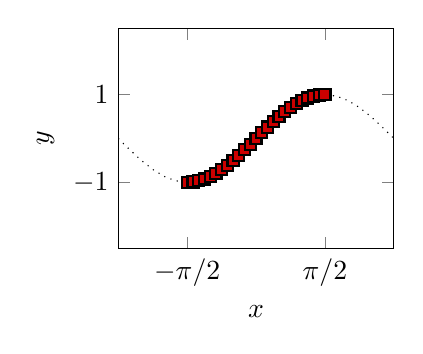
\begin{tikzpicture}
          \begin{axis}[width = 2in,
            xmin=-pi, xmax=pi, ymin=-1.2,ymax=1.2,
            xtick={-pi/2,pi/2}, xticklabels={$-\pi/2$,$\pi/2$},
            ytick={-1,1}, xlabel=$x$, ylabel=$y$, axis equal=true]
            \addplot[domain=-pi:pi,dotted,black]{sin(deg(x))};
            \addplot+[domain=-pi/2:pi/2,thick,black]{sin(deg(x))};
          \end{axis}
        \end{tikzpicture}
        &
        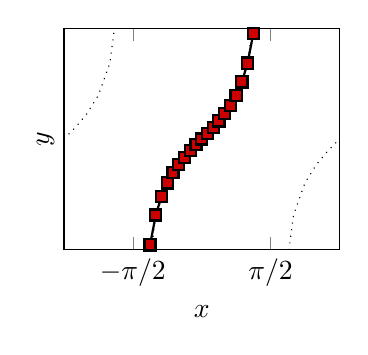
\begin{tikzpicture}
          \begin{axis}[width = 2in,
            xmin=-pi, xmax=pi, ymin=-1.2,ymax=1.2,
            extra x ticks={-pi/2,pi/2}, extra x tick labels={$-\pi/2$,$\pi/2$},
            ytick=\empty, xtick = \empty, xlabel=$x$, ylabel=$y$, axis equal=true,
            restrict y to domain=-10:10]
            \addplot[domain=-pi:pi,dotted,black]{tan(deg(x))};
            \addplot+[domain=-pi/2:pi/2,thick,black]{tan(deg(x))};
          \end{axis}
        \end{tikzpicture}
        \\
        $\cos x$ on $[0,\pi]$ &
        $\sin x$ on $[-\frac{\pi}{2},\frac{\pi}{2}]$ &
        $\tan x$ on $[-\frac{\pi}{2},\frac{\pi}{2}]$
    \end{tabular}
    \end{center}
    \item Definitions:
      \begin{itemize}[topsep=0pt]
        \item $\arccos x$ is the angle in the interval $[0, \pi]$ whose cosine is $x$.

        $\arccos$ takes inputs in $\fitb{1in}{[{-1}, 1]}$ 
        and spits out numbers between $\fitb{1in}{[0, \pi]}$.
        
        \item $\arcsin x$ is the angle in the interval $[{-\frac{\pi}{2}},
        \frac{\pi}{2}]$ whose sine is $x$.

        $\arcsin$ takes inputs in $\fitb{1in}{[{-1}, 1]}$ 
        and spits out numbers between $\fitb{1in}{[{-\frac{\pi}{2}},
        \frac{\pi}{2}]}$.
        
        \item $\arctan x$ is the angle in the interval $({-\frac{\pi}{2}},
        \frac{\pi}{2})$ whose tangent is $x$.

        $\arctan$ takes inputs in $\fitb{1in}{({-\infty}, \infty)}$ 
        and spits out numbers between $\fitb{1in}{({-\frac{\pi}{2}},
        \frac{\pi}{2})}$.
      \end{itemize}
\end{itemize}
\end{framed}

\end{document}